\documentclass[tikz,border=10pt]{standalone}
% Scale s = 0.009988 cm/px, centred on ink bbox (cx=457, cy=252); y flipped
\begin{document}
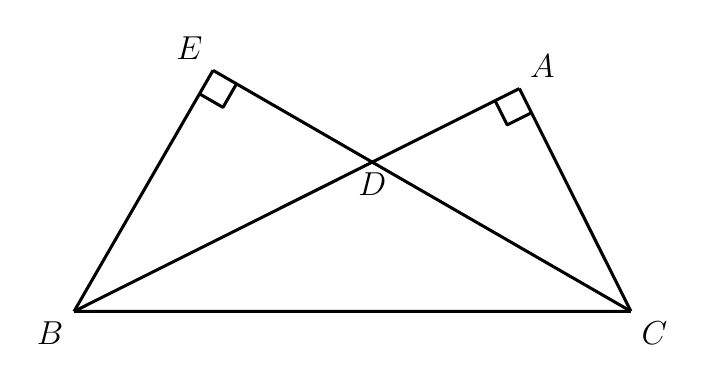
\begin{tikzpicture}[line width=1.1pt, line join=round]
  % Named vertices (converted from pixels)
  \coordinate (B) at (-3.531276834205261,-1.526966465398236);
  \coordinate (C) at (3.540739846582424,-1.5254214747091959);
  \coordinate (D) at (0.256353597203039,0.368747299072797);
  \coordinate (A) at (2.124685949489699,1.3038499763209201);
  \coordinate (E) at (-1.7655025590699007,1.5347906647137148);

  % Right-angle mark at A (corner square: arms A->P1, A->P3, far corner P2)
  \coordinate (PA1) at (1.815837934310496,1.1505532586180132);
  \coordinate (PA2) at (1.9699590568984098,0.8421115645600352);
  \coordinate (PA3) at (2.2778085968832587,0.9954080819898963);

  % Right-angle mark at E
  \coordinate (QE1) at (-1.467682043696476,1.3634803224920766);
  \coordinate (QE2) at (-1.6392028938947454,1.06420234873461);
  \coordinate (QE3) at (-1.9380232094163865,1.2365142222002665);

  % Solid segments
  \draw (B) -- (C);
  \draw (B) -- (A);   % passes through D
  \draw (E) -- (C);   % passes through D
  \draw (E) -- (B);
  \draw (A) -- (C);

  % Right-angle marks (drawn inside the triangles)
  \draw (PA1) -- (PA2) -- (PA3);
  \draw (QE1) -- (QE2) -- (QE3);

  % Labels
  \node[above right] at (A) {\fontsize{11.5}{13.8}\selectfont $A$};
  \node[below left]  at (B) {\fontsize{11.5}{13.8}\selectfont $B$};
  \node[below right] at (C) {\fontsize{11.5}{13.8}\selectfont $C$};
  \node[below]       at (D) {\fontsize{11.5}{13.8}\selectfont $D$};
  \node[above left]  at (E) {\fontsize{11.5}{13.8}\selectfont $E$};
\end{tikzpicture}
\end{document}
% GEOAGENT_REPAIR_V1 c18a466396f54661 11e90abeead3ebb0e86a1592b6a3299b85e5d68706ffbe7714c08f68f76f130a